\documentclass[conference]{IEEEtran}

\usepackage{amsmath,amssymb}
\usepackage{booktabs}
\usepackage{graphicx}
\usepackage{url}
\usepackage{multirow}
\usepackage{xcolor}
\usepackage{balance}
\usepackage{tikz}
\usetikzlibrary{arrows.meta,positioning,shapes.geometric}

\title{Spatial-Context-Aware Sequential Pattern Mining for Financial Fraud Detection Using the IEEE-CIS Dataset}

\author{
\IEEEauthorblockN{Gladwin Daniel P, Karthikeyan A, and Srishreyan}
\IEEEauthorblockA{VIT Chennai\\
Chennai, India}
}

\begin{document}
\maketitle

\begin{abstract}
Financial fraud is a highly imbalanced and evolving classification problem in which transaction order, timing, identity context, and location-related signals may jointly indicate malicious behavior. This paper presents a spatial-context-aware sequential pattern mining framework for the IEEE-CIS Fraud Detection dataset. The framework first constructs user transaction sequences and spatial transaction clusters, then uses cluster-specific adaptive support thresholds for PrefixSpan mining. To connect the mined sequential evidence with spatial context at classification time, we introduce Contextual Trajectory Surprise (CTS), a feature block containing risk-weighted sequence surprise, user spatial-cluster switching, and user-specific distance inconsistency. CatBoost is used as the primary hybrid classifier, while XGBoost, Random Forest, and Logistic Regression provide comparison baselines. On the current 100,000-row chronological experiment, CTS with CatBoost achieved ROC-AUC 0.8919, PR-AUC 0.5576, F1-score 0.2579, and precision@top-10\% of 0.1610. These results exceed the implemented standalone and previous XGBoost hybrid baselines. The contribution is positioned as a proposed and interpretable combination of spatially conditioned pattern mining and trajectory-level interaction features; it is not claimed to be universally unprecedented. A leakage-controlled evaluation using training-only risk estimates and pattern libraries is identified as essential future validation.
\end{abstract}

\begin{IEEEkeywords}
financial fraud detection, sequential pattern mining, PrefixSpan, DBSCAN, CatBoost, spatial context, anomaly detection, IEEE-CIS
\end{IEEEkeywords}

\section{Introduction}
Electronic commerce produces transaction streams in which fraudulent activity can appear as an unusual sequence of amounts, products, time gaps, devices, or locations. The difficulty is increased by class imbalance: a detector must identify a small number of fraudulent transactions without overwhelming investigators with false alerts. A model that uses only independent transaction attributes may miss behavioral structure, while a purely sequential model may ignore contextual differences between transaction regions or address populations.

This work studies the following question: can spatial context improve sequential fraud signals when the two are connected before supervised classification? The proposed pipeline uses address and distance proxies from the IEEE-CIS dataset to create density-based clusters. Each cluster receives a fraud-risk estimate and an adaptive minimum-support threshold for sequential pattern mining. The resulting anomaly signal is augmented with CTS features that represent the interaction between behavioral surprise and local spatial context.

The main contributions are:
\begin{enumerate}
    \item a spatially conditioned PrefixSpan procedure that creates cluster-specific frequent-pattern libraries;
    \item the CTS feature block, which combines contextual sequence surprise, spatial switching, and user-specific distance inconsistency;
    \item an interpretable CatBoost-based hybrid classifier evaluated against XGBoost, Random Forest, and Logistic Regression baselines; and
    \item an explicit evaluation protocol and limitation statement for preventing overclaiming under temporal and label leakage risks.
\end{enumerate}

\begin{figure*}[t]
\centering
\resizebox{\textwidth}{!}{%
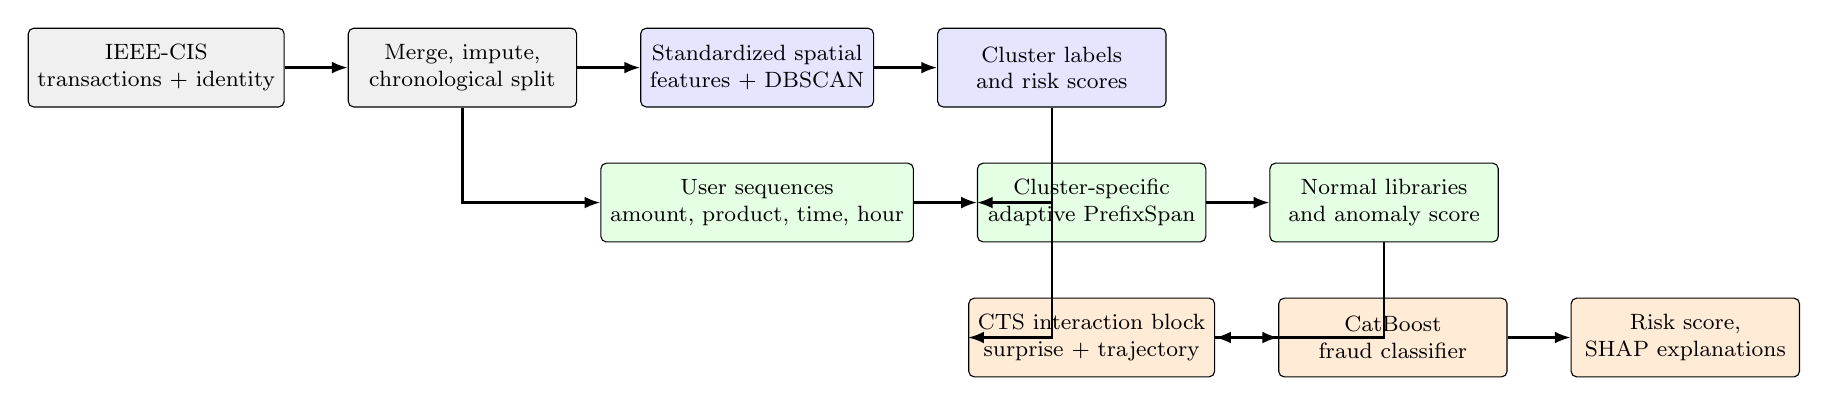
\begin{tikzpicture}[
    node distance=7mm and 8mm,
    block/.style={draw, rounded corners=2pt, align=center, minimum height=10mm, minimum width=29mm, font=\footnotesize},
    data/.style={block, fill=gray!12},
    spatial/.style={block, fill=blue!10},
    sequential/.style={block, fill=green!10},
    model/.style={block, fill=orange!16},
    arrow/.style={-{Latex[length=2mm]}, thick}
]
\node[data] (raw) {IEEE-CIS\\transactions + identity};
\node[data, right=of raw] (prep) {Merge, impute,\\chronological split};
\node[spatial, right=of prep] (dbscan) {Standardized spatial\\features + DBSCAN};
\node[spatial, right=of dbscan] (risk) {Cluster labels\\and risk scores};
\node[sequential, below=of dbscan] (seq) {User sequences\\amount, product, time, hour};
\node[sequential, right=of seq] (prefix) {Cluster-specific\\adaptive PrefixSpan};
\node[sequential, right=of prefix] (anom) {Normal libraries\\and anomaly score};
\node[model, below=of prefix] (cts) {CTS interaction block\\surprise + trajectory};
\node[model, right=of cts] (cat) {CatBoost\\fraud classifier};
\node[model, right=of cat] (out) {Risk score,\\SHAP explanations};
\draw[arrow] (raw) -- (prep);
\draw[arrow] (prep) -- (dbscan);
\draw[arrow] (dbscan) -- (risk);
\draw[arrow] (prep) |- (seq);
\draw[arrow] (risk) |- (prefix);
\draw[arrow] (seq) -- (prefix);
\draw[arrow] (prefix) -- (anom);
\draw[arrow] (risk) |- (cts);
\draw[arrow] (anom) |- (cts);
\draw[arrow] (cts) -- (cat);
\draw[arrow] (cat) -- (out);
\end{tikzpicture}}
\caption{End-to-end spatial-context-aware sequential fraud detection framework.}
\label{fig:pipeline}
\end{figure*}

\section{Related Work and Research Positioning}
Sequential learning has been applied to payment fraud by modeling transaction order and user behavior. Markov and recurrent approaches can represent temporal dependencies, while sequential pattern mining provides human-readable recurring behavior. PrefixSpan is particularly useful for mining frequent subsequences without generating the full candidate set first \cite{pei2001prefixspan}. Spatial and density-based methods, including DBSCAN, are useful for identifying local transaction populations and outliers, but spatial clustering alone does not express the order of events.

Graph-based fraud detection is an important international comparison family. Temporal graph and causal temporal graph models represent relational and time-dependent behavior; for example, CaT-GNN combines temporal graph learning with causal intervention for fraud detection \cite{duan2024catgnn}. Such methods motivate graph-based future baselines but do not directly replace the interpretable pattern-library design used here. A commonly cited survey also emphasizes class imbalance, changing fraud behavior, and the importance of feature construction in credit-card fraud detection \cite{abdallah2016survey}.

Recent India-focused search results similarly emphasize graph neural networks, adaptive risk scoring, and digital-payment fraud detection. However, the present dataset is the public IEEE-CIS benchmark rather than an India-specific payment dataset. Therefore, the claim made here is deliberately narrow: CTS plus spatially conditioned PrefixSpan is proposed as a differentiated, interpretable design for this benchmark. A systematic review across IEEE Xplore, ACM Digital Library, Scopus, Web of Science, and Indian indexing sources is required before making a priority claim.

\section{Dataset and Preprocessing}
The IEEE-CIS Fraud Detection dataset contains approximately 590,540 labeled transactions with transaction and identity tables. This implementation uses a 100,000-row time-ordered sample for rapid experimentation. Transaction and identity records are merged on \texttt{TransactionID}. Missing address values are imputed with the mode, distance values with the median, count features with zero, and identity values with explicit missing indicators or an ``unknown'' category.

A composite user key is constructed from \texttt{card1}, \texttt{addr1}, and \texttt{P\_emaildomain}. Transactions are ordered by \texttt{TransactionDT}. The chronological first 80\% is used for training and the final 20\% for testing. The observed training fraud rate is 2.66\%, while the test fraud rate is 2.18\% in the current sample.

For sequential mining, each transaction is represented by a tuple containing an amount bin, product category, time-delta bin, and hour of day. Amounts are discretized into eight ranges and time gaps into six ranges. This representation trades numerical detail for interpretable sequential items.

\section{Proposed Framework}
\subsection{Spatial Clustering}
The spatial feature vector is
\begin{equation}
\begin{aligned}
    \mathbf{s}_i = [&\operatorname{enc}(addr1_i),\operatorname{enc}(addr2_i),\\
    &\operatorname{norm}(dist1_i),\operatorname{norm}(dist2_i)].
\end{aligned}
\end{equation}
The encoded and normalized vectors are standardized and clustered with DBSCAN. The epsilon value is estimated from a k-distance distribution and constrained to a practical range. Noise points are assigned to their nearest non-noise cluster using a 1-nearest-neighbor rule.

For cluster $c$, the risk score is calculated as
\begin{equation}
    R_c = \frac{\operatorname{fraud\ rate}(c)}{\operatorname{global\ fraud\ rate}}.
\end{equation}

\subsection{Spatially Conditioned Sequential Mining}
User sequences are grouped by their dominant spatial cluster. PrefixSpan is run independently for each cluster. The adaptive support fraction is
\begin{equation}
    \sigma_c = \operatorname{clip}\left(\sigma_0 \frac{1}{R_c},
    \sigma_{min}, \sigma_{max}\right),
\end{equation}
where $\sigma_0$ is the base support, and the implementation uses a 0.01 floor and a 0.20 ceiling. High-risk clusters therefore admit less frequent patterns, while low-risk clusters require stronger recurrence.

For a user sequence $q$, the anomaly score compares the sequence with the normal pattern library of its assigned cluster:
\begin{equation}
    A(q,c) = 1 - \frac{\max\{support(p):p\subseteq q,\ p\in L^{normal}_c\}}
    {\max\{support(p):p\in L^{normal}_c\}}.
\end{equation}
Here, $p\subseteq q$ denotes a subsequence match. A high value indicates weak agreement with the normal cluster-specific library.

\subsection{Contextual Trajectory Surprise}
The original spatial and sequential outputs are scalar columns. CTS adds interaction and trajectory information:
\begin{align}
    C_i &= A_i\left(1+\log(1+R_i)\right),\\
    S_i &= \mathbb{1}(cluster_i\ne cluster_{i-1}),\\
    \bar{S}_u &= \operatorname{mean}_{i\in u}(S_i),\\
    D_i &= \left|\bar{d}_i-\operatorname{median}_{j\in u}(\bar{d}_j)\right|,
\end{align}
where $\bar{d}_i$ is the mean of the normalized distance features for transaction $i$. The features are named \texttt{contextual\_surprise}, \texttt{spatial\_switch}, \texttt{spatial\_switch\_rate}, and \texttt{spatial\_inconsistency}.

\subsection{Classification and Explainability}
CatBoost is the primary classifier because the final feature table contains nonlinear interactions and many categorical-derived or missing-value-derived variables. Class balancing is handled using CatBoost's balanced class-weight option. XGBoost is retained as the main gradient-boosting ablation, with Random Forest and Logistic Regression as additional comparisons.

\begin{figure}[t]
\centering
\resizebox{\columnwidth}{!}{%
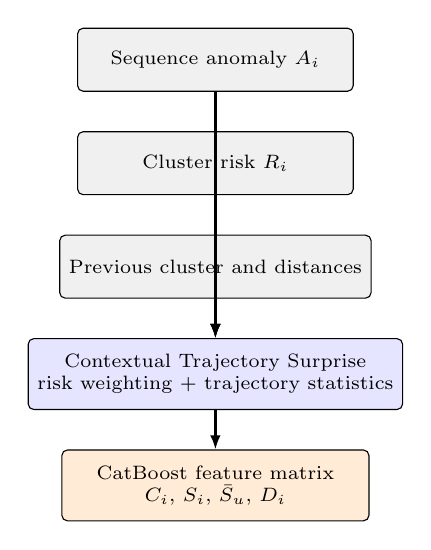
\begin{tikzpicture}[
    node distance=5mm,
    input/.style={draw, rounded corners=2pt, align=center, minimum width=35mm, minimum height=8mm, font=\scriptsize, fill=gray!12},
    operation/.style={draw, rounded corners=2pt, align=center, minimum width=39mm, minimum height=9mm, font=\scriptsize, fill=blue!10},
    output/.style={draw, rounded corners=2pt, align=center, minimum width=39mm, minimum height=9mm, font=\scriptsize, fill=orange!16},
    arrow/.style={-{Latex[length=1.8mm]}, thick}
]
\node[input] (a) {Sequence anomaly $A_i$};
\node[input, below=of a] (r) {Cluster risk $R_i$};
\node[input, below=of r] (s) {Previous cluster and distances};
\node[operation, below=of s] (fuse) {Contextual Trajectory Surprise\\risk weighting + trajectory statistics};
\node[output, below=of fuse] (features) {CatBoost feature matrix\\$C_i$, $S_i$, $\bar S_u$, $D_i$};
\draw[arrow] (a) -- (fuse);
\draw[arrow] (r) -- (fuse);
\draw[arrow] (s) -- (fuse);
\draw[arrow] (fuse) -- (features);
\end{tikzpicture}}
\caption{CTS transforms separate spatial and sequential evidence into interaction features.}
\label{fig:cts}
\end{figure}

SHAP TreeExplainer is used to generate global feature-importance plots and cluster-specific explanations for the CatBoost model. These explanations are intended to show whether contextual surprise, spatial risk, raw transaction variables, or identity variables drive predictions. SHAP analysis was not generated in the reported run because the active runtime lacked the SHAP package; it remains part of the reproducible implementation and should be regenerated after installing the dependency in the active environment.

\section{Experimental Design}
The evaluation uses the chronological 80/20 split and reports ROC-AUC, PR-AUC, F1-score, precision, recall, and precision at the top 10\% of investigation candidates. PR-AUC and precision@top-10\% are emphasized because ROC-AUC can appear strong under severe class imbalance.

Four feature/model conditions are compared. The baseline uses raw features only. Sequential-only includes the anomaly score but removes spatial and CTS columns. Spatial-only includes spatial columns but removes anomaly and CTS columns. The proposed hybrid uses the full feature matrix and CatBoost. The first three conditions are retrained with XGBoost to isolate the contribution of the proposed hybrid design from the change in classifier.

\begin{figure}[t]
\centering
\resizebox{\columnwidth}{!}{%
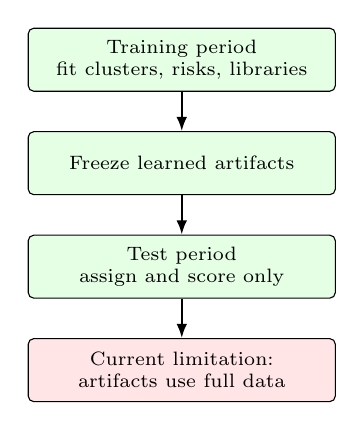
\begin{tikzpicture}[
    node distance=5mm,
    block/.style={draw, rounded corners=2pt, align=center, minimum width=39mm, minimum height=8mm, font=\scriptsize},
    safe/.style={block, fill=green!10},
    warning/.style={block, fill=red!10},
    arrow/.style={-{Latex[length=1.8mm]}, thick}
]
\node[safe] (train) {Training period\\fit clusters, risks, libraries};
\node[safe, below=of train] (freeze) {Freeze learned artifacts};
\node[safe, below=of freeze] (test) {Test period\\assign and score only};
\node[warning, below=of test] (current) {Current limitation:\\artifacts use full data};
\draw[arrow] (train) -- (freeze);
\draw[arrow] (freeze) -- (test);
\draw[arrow] (test) -- (current);
\end{tikzpicture}}
\caption{Evaluation boundary and the leakage-control requirement.}
\label{fig:validity}
\end{figure}

\begin{table}[t]
\caption{Results on the Current 100K-Row Chronological Experiment}
\label{tab:results}
\centering
\scriptsize
\begin{tabular}{lccccc}
\toprule
Model & ROC-AUC & PR-AUC & F1 & Recall & P@10\% \\
\midrule
Baseline XGBoost & 0.8836 & 0.5149 & 0.2320 & 0.7408 & 0.1580 \\
Sequential-only & 0.8824 & 0.5229 & 0.2278 & 0.7408 & 0.1580 \\
Spatial-only & 0.8829 & 0.5287 & 0.2416 & 0.7225 & 0.1540 \\
CTS + CatBoost & \textbf{0.8919} & \textbf{0.5576} & \textbf{0.2579} & 0.7477 & \textbf{0.1610} \\
\bottomrule
\end{tabular}
\end{table}

\section{Results and Discussion}
The CTS + CatBoost hybrid obtains the strongest result in every ranking-oriented metric in Table~\ref{tab:results}. Relative to the previous CTS + XGBoost run, PR-AUC increases from 0.5418 to 0.5576 and ROC-AUC increases from 0.8866 to 0.8919. Relative to spatial-only XGBoost, PR-AUC increases by 0.0289 and F1 increases by 0.0163.

The improvement supports the hypothesis that sequential surprise becomes more useful when conditioned on spatial risk and user trajectory behavior. It does not prove that CatBoost or CTS will improve every dataset or split. The current experiment is a single sample and chronological split, so confidence intervals, repeated time windows, and a full-dataset run are required for a stronger conclusion.

\section{Threats to Validity and Reproducibility}
The current implementation has an important leakage risk. Spatial cluster risk scores and sequential pattern libraries are generated before the train/test split, which can allow test-period labels or behavior to influence training features. In a publication-grade experiment, spatial clusters may be fit using training data, cluster risk must use training labels only, and PrefixSpan libraries must be mined from training sequences only. Test transactions should then be assigned to learned clusters and scored against frozen training libraries.

The address fields are geographic proxies rather than coordinates, so DBSCAN clusters should not be interpreted as literal maps. The 100,000-row time-ordered sample may also differ from the full competition distribution. Finally, the current paper reports predictive metrics but not confidence intervals, threshold calibration, latency, or cost-weighted business utility.

\section{Conclusion}
This paper presented a spatial-context-aware sequential fraud detection framework using DBSCAN, adaptive PrefixSpan mining, CTS interaction features, and CatBoost classification. On the current experiment, the proposed hybrid outperformed the implemented sequential-only, spatial-only, and baseline XGBoost models. The main research contribution is the interpretable connection between local spatial risk, sequential pattern surprise, and user trajectory inconsistency. The next evaluation step is leakage-controlled retraining using training-only artifacts, followed by repeated temporal validation and SHAP-based analysis in the active runtime.

\section*{Acknowledgment}
The authors are students of VIT Chennai. The experiments use the IEEE-CIS Fraud Detection dataset released through the Kaggle competition.

\balance
\begin{thebibliography}{00}
\bibitem{pei2001prefixspan} J. Pei, J. Han, B. Mortazavi-Asl, H. Pinto, Q. Chen, U. Dayal, and M.-C. Hsu, ``PrefixSpan: Mining sequential patterns efficiently by prefix-projected pattern growth,'' \textit{IEEE Transactions on Knowledge and Data Engineering}, vol. 16, no. 11, pp. 1424--1440, 2004.

\bibitem{jurgovsky2018sequence} J. Jurgovsky, M. Granitzer, K. Ziegler, S. Calabretto, P. Portier, L. He-Guelton, and O. Caelen, ``Sequence classification for credit-card fraud detection,'' \textit{Expert Systems with Applications}, vol. 100, pp. 234--245, 2018.

\bibitem{abdallah2016survey} A. Abdallah, M. A. Maarof, and A. B. Zainal, ``Fraud detection system: A survey,'' \textit{Journal of Network and Computer Applications}, vol. 68, pp. 90--113, 2016.

\bibitem{duan2024catgnn} Y. Duan, G. Zhang, S. Wang, X. Peng, W. Ziqi, J. Mao, H. Wu, X. Jiang, and K. Wang, ``CaT-GNN: Enhancing credit card fraud detection via causal temporal graph neural networks,'' arXiv:2402.14708, 2024. [Online]. Available: \url{https://arxiv.org/abs/2402.14708}

\bibitem{ieeecis} Vesta Corporation, ``IEEE-CIS Fraud Detection,'' Kaggle competition dataset, 2019. [Online]. Available: \url{https://www.kaggle.com/c/ieee-fraud-detection}
\end{thebibliography}

\end{document}
